\documentclass[a4paper,11pt]{article}
\usepackage{amssymb}
\usepackage{booktabs}
\usepackage{geometry}
\usepackage{color}
\usepackage{hyperref}
\usepackage{listings}
\usepackage{graphicx}
\usepackage{float}
\usepackage{caption}
\usepackage{subcaption}
\usepackage[T1]{fontenc}

\catcode`\^^I=13
\catcode`\^^M=13

\newcounter{linenumber}

\newenvironment{sourcecode}{\begingroup%
\setcounter{linenumber}{0}%
\def\algorithm##1{\setcounter{linenumber}{0}\medskip \textbf{Algorithm} \textsc{##1} \parskip=0pt\everypar={\parskip=0pt\stepcounter{linenumber}\rlap{\scriptsize{\thelinenumber}}\qquad}}%
\def\event##1{\setcounter{linenumber}{0}\medskip \textbf{##1:} \parskip=0pt\everypar={\parskip=0pt\stepcounter{linenumber}\rlap{\scriptsize{\thelinenumber}}\qquad}}%
%
\def\comment##1{\textit{//##1}}%
\def\qif##1{\textbf{if} ##1}%
\def\qifdefined##1{\textbf{if} ##1 \textbf{defined}}%
\def\qifndefined##1{\textbf{if} ##1 \textbf{not defined}}%
\def\qelse{\textbf{else}}%
\def\qelseif##1{\textbf{else if ##1}}%
\def\for##1{\textbf{for} ##1}%
\def\foreach##1{\textbf{for each} ##1}%
\def\qdo{\textbf{do}}%
\def\while##1{\textbf{while} ##1}%
\def\return##1{\textbf{return} ##1}%
\def\break{\textbf{break}}%
\def\qglobal##1{\textbf{global} ##1}%
\def\qsend##1{\textbf{send} \emph{##1}}%
\def\qreceive##1{\textbf{receive} \emph{##1}}%
\def\qbegin{\textbf{begin}}
\def\qend{\everypar={}\textbf{end}}
\def\runningtime##1{\hfill ##1}
\catcode`\^^I=13%
\catcode`\^^M=13%
\def^^I{\qquad}%
\def^^M{\par}%
}{\endgroup}

\catcode`\^^I=10
\catcode`\^^M=5


\graphicspath{{img/}}

\setlength\parindent{0cm}

\geometry{
	includeheadfoot,
	margin=2.54cm
}

\title{
	2IL76 Algorithms for Geographic Data Set 1 \\
}
\author{
	Tim van Dalen (0744839)
	\and
	Bram Kohl (0746107)
	\and
	Bart van Wezel (0740608)
}
\date{\today}

\begin{document}
	\maketitle
	
\section*{Exercise 3}
We came up with a measure for how close a polygonal curve Q is to a point set P.

We define the distance of a point in P to a line segment in Q as the minimum of the perpendicular distance to the line segment and the Euclidian distances to the two endpoints of the line segment.
We define the perpendicular distance to the line segment as the perpendicular distance to the line through the endpoints of the line segments, or infinite if the intersection point of the perpendicular line with the line through the endpoints is not on the line segment.
See for example Figure~\ref{fig:perp-distance}.

Here, the perpendicular distance is infinite as $Q_I$ is not on the line segment ($Q_1,Q_2$).

\begin{figure}[H]
	\centering
	\def\svgwidth{0.5\textwidth}
	\input{img/perp-distance.pdf_tex}
	\caption{Infinite perpendicular distance}
	\label{fig:perp-distance}
\end{figure}

As not all points have to be close, we came up with a formula that defines the number of nearest points in P we will be looking at for each line segment.
We do this in order to reduce noise from outliers.
The formula we came up with is: $\lceil n\cdot \frac{l}{tl}\rceil$ where $n = |P|$, $l$ is the length of the line segment in Q we are currently looking at and $tl$ is the total length of the line segments in Q.
This way, longer lines need more close points than shorter lines.
Note that when adding the number of nearest points for each line segment you get $n$, but this does not mean all points have to be one of the nearest points of a line segment, as a point can be a nearest point for multiple line segments.

We wanted large line segments to take into consideration more nearest neighbours than small line segments because this is useful when P is well distributed over Q.
See for example figure \ref{fig:line-weight}. In this figure $n = 14$ and the line segments are of length 1, 1 and 8. So for the line segments of length 1 we look at the nearest $\lceil 14\cdot \frac{1}{10}\rceil = 2$ points and for the line segment of length 8 we look at the nearest $\lceil 14\cdot \frac{8}{10}\rceil = 12$ points. This way, long line segments need more points.

\begin{figure}[H]
	\centering
	\def\svgwidth{0.5\textwidth}
	\input{img/line-weight.pdf_tex}
	\caption{A point set P that is well distributed over curve Q}
	\label{fig:line-weight}
\end{figure}

 
	We assume the following two simple helper algorithms:

\begin{description}
	\item[\textsc{PerpDistance}($p$, $(q_i, q_j)$)] calculates the perpendicular distance from point $p$ to line segment $(q_i, q_j)$.
		If there is no such distance (because the perpendicular line from $p$ to the line that $(q_i, q_j)$ lies on does not cross $(q_i, q_j)$), this algorithm returns $\infty$.
	\item[\textsc{PointDistance}($p$, $q$)] calculates the Euclidean distance between points $p$ and $q$.
	\item[\textsc{LineSegLength}($(q_i, q_j)$)] calculates the length of a line segment
	\item[\textsc{LineLength}($Q$)] calculates the sum of the lengths of all line segments in a line
\end{description}

\begin{sourcecode}
\algorithm{Distance($p$, $(q_i, q_j)$}
\return{$\min\left(\textsc{PerpDistance}(p, (q_i, q_j)), \textsc{PointDistance}(p, q_i), \textsc{PointDistance}(p, q_j)\right)$}
\qend

\algorithm{SegmentMetric($(q_i, q_j)$, $P$, $Q$)}
$D$ is a map from point to distance to that point
\foreach{point $p$ in $P$}
	$D[p]$ = \textsc{Distance}($p$, $(q_i, q_j)$)
|
\return{the sum of the $\lceil |P| \frac{\textsc{LineSegLength}((q_i, q_j))}{\textsc{LineLength}(Q)} \rceil$ lowest distances in $D$}
\qend

\algorithm{PointCurveDistanceMetric($P$, $Q$)}
$\phi = 0$
\foreach{line segment $(q_i, q_j)$ in $Q$}
	$\phi = \phi + $ \textsc{SegmentMetric}($(q_i, q_j)$, $P$, $Q$)
|
\return{\phi}
\qend
\end{sourcecode}

	
We will now analyse the running time of the algorithm. 
We will do this by analysing the running time of each function.\\
\textsc{PerpDistance}($p$, $(q_i, q_j))$ takes $O(1)$ time.\\
\textsc{PointDistance}($p$, $q$) takes $O(1)$ time. \\
\textsc{LineSegLength}($(q_i, q_j)$) takes $O(1)$ time. \\
\textsc{LineLength}($Q$) takes $O(m)$ time, but if we cache the result, we only have to calculate it once. This means that when this function is called multiple times it will not become $\cdot m$ , but $+m$.\\
\textsc{Distance}($p$, $(q_i, q_j)$) takes $O(1)$ time.\\
\textsc{SegmentMetric}(($(q_i, q_j)$, $P$, $Q$) takes $O(n+m)$ time, because there is a for loop over n points. \\
\textsc{PointCurveDistanceMetric}($P$, $Q$)  takes $O(mn + m)$ time, which is $O(mn)$. 
There is a loop of m segments over a function, that takes $O(n+m)$ time, but the $m$ in that function is only calculated once, so it stays $O(mn+m)$ time and not $O(m(n+m))$ time.
So the running time of our algorithm is  $O(mn)$ \\

The measure should give a low value for the distance when everywhere on Q, there are several points of P close by, and a higher value when more or longer parts of Q do not have several points close by.
However in the following example Figure~\ref{fig:example1}. Each line segment has points close by. 
The points above the long line segments are still pretty close to the long line, but there is still a longer part of Q that does not have points close by. 
We do take the length of the lines in acccount, but we do not look where those points are on each line segment. 
So our algorithm returns false values when there are long line segments which have points close by, but those points are all close to one point on that line and not nicely distributed. 
\begin{figure}[H]
	\centering
	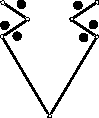
\includegraphics[width=0.5\textwidth]{img/example1.pdf}
	\caption{A line Q and points P, for which our algorithm gives a low value, but should return a high value.}
	\label{fig:example1}
\end{figure}



\end{document}
